\documentclass[12pt]{report}

\usepackage{commands}


\begin{document}

\large

\begin{center}
 Math 575 Homework 2\\
 Due April 26\\
 By Marvyn Bailly\\
\end{center}

\normalsize

\hrule

%---------------%
%---Problem 1---%
%---------------%

%--status--$

\begin{problem}
    Project preparation!
    \begin{enumerate}
        \item [(a)] Provide the citation for the paper you're planning to base your presentation on, and a list of your planned group members.  
        \item [(b)]  Write two sentences describing the main techniques from dynamical systems, broadly interpreted, used in the paper.  
        \item[(c)]  Write two sentences describing the conclusions that the paper found.  
        \item[(d)]  Write one sentence with an idea for a possible extension to the paper that you might explore.
    \end{enumerate}
\end{problem}

\begin{solution}

    \noindent
    \begin{enumerate}
        \item Our group members are 
        \begin{itemize}
            \item Charbel Abi Younes,

            \item Marvyn Bailly,

            \item Bart Boom,

            \item Rohin Gilman,

            \item Daran Xu.
        \end{itemize}
        We are referencing the paper \emph{Bayesian Learning and Inference in
        Recurrent Switching Linear Dynamical Systems} by Scott Linderman: \\

        
        Linderman, S., Johnson, M., Miller, A., Adams, R., Blei, D. \&; Paninski, L.. (2017). Bayesian Learning and Inference in Recurrent Switching Linear Dynamical Systems. \emph{Proceedings of the 20th International Conference on Artificial Intelligence and Statistics}, in \emph{Proceedings of Machine Learning Research} 54:914-922 
        
        Available from https://proceedings.mlr.press/v54/linderman17a.html. \\
        

        \item This paper describes how a switching linear dynamical system (SLDS) can be prescribed to a problem to learn its dynamics. In particular, the paper examines recurrent SLDS (rSLDS), a variation on standard SLDS in which, as opposed to merely the discrete state as in conventional SLDS, the subsequent discrete latent state depends on both the current discrete and continuous latent states.

        \item In order to make the posterior distribution follow a Gaussian distribution, the paper establishes that one can construct a conjugate pair by including an auxiliary variable. This benefit suggests that rLSDS is able to more accurately capture the maximum amount of time spent in the high probability side of the Lorenz's system. 

        \item We would like to explore a simple, yet interesting, dynamical system (such as the Van der Pol Oscillator or double pendulum) that has bifurcations to see how this rSLDS model responds to these bifurcations.

    \end{enumerate}



\end{solution}

%----------------------------------------------------------------------------------------------------%
%\vskip 20pt
\newpage


%---------------%
%---Problem 2---%
%---------------%

%--status--$

\begin{problem}
    Consider the dipole system again

\begin{equation}
\left\{\begin{array}{l}
\dot x= x^2 - y^2  \\
\dot y = 2 x y 
\end{array}\right.
\end{equation}

\begin{enumerate}
    \item [(a)] What is the center manifold (and what is its dimension)?  
    \item [(b)] Find a one-dimensional invariant manifold. 
\end{enumerate}
\end{problem}

\begin{solution}

    \noindent
    Consider the dipole system
    \[ 
    \left\{\begin{array}{l}
    \dot x= x^2 - y^2,  \\
    \dot y = 2 x y.
    \end{array}\right.
    \]
    \begin{enumerate}
        \item [(a)] 
        We wish to find the center manifold and its dimension. We begin by finding the fixed point of this system to be $(0,0)$. Next we compute the Jacobian to be
        \[ 
            J(x,y) = \begin{bmatrix}
                2x & -2y\\
                2y & 2x
            \end{bmatrix}.
        \]
        Thus the Jacobian at the fixed point is
        \[ 
            J(0,0) = \begin{bmatrix}
                0 & 0 \\ 0 & 0
            \end{bmatrix},
        \]
        which has an eigenvalue of $\lambda_1$ with multiplicity two and eigenvectors $(1,0)^T$ and $(0,1)^T$ which are orthogonal and span $\R^2$. Thus the center manifold, $W^c$, is described by the eigenvector space and is dimension $2$. 
        
        \item [(b)] We can find a one-dimensional invariant manifold by observing that on the line $y=0$, we have $y_t=0$ and thus trajectory along $y=0$ stay on $y=0$. Thus we have found an one-dimensional invariant manifold defined by $y=0$.
    \end{enumerate}
\end{solution}

%----------------------------------------------------------------------------------------------------%
%\vskip 20pt
\newpage


%---------------%
%---Problem 3---%
%---------------%

%--status--$

\begin{problem}
    Consider the system 
\begin{equation}
\left\{\begin{array}{l}
\dot x= -x \\
\dot y = y + \alpha x^3 
\end{array}\right.
\end{equation}
for $\alpha>0$.  Find an exact expression for the global stable and unstable manifolds (i.e., not in terms of a polynomial expansion).
\end{problem}

\begin{solution}

    \noindent
    Consider the system 
    \begin{equation}
        \left\{\begin{array}{l}
        \dot x= -x \\
        \dot y = y + \alpha x^3 
        \end{array}\right.
    \end{equation}
    for $\alpha>0$. This system has a fixed point at $(0,0)$ and we can compute the Jacobian to be
    \[ 
        J(x,y) = \begin{bmatrix}
            -1 & 0\\
            3\alpha x^2 & 1\\
        \end{bmatrix},
    \]
    and evaluating the Jacobian at the fixed point yields
    \[ 
        J(0,0) = \begin{bmatrix}
            -1 & 0 \\
            0 & 1
        \end{bmatrix}.
    \]
    The eigenvalues of $J(0,0)$ are $\lambda_1 = -1$ and $\lambda_2 = 1$ which have eigenvectors $v_1 = (1,0)^T$ and $v_2 = (0,1)^T$ respectively. Since the system is 2-dimensional, we know the eigenpairs represent the global stable and unstable manifolds and must be one-dimensional respectively. Thus the span of $v_1$ describe stable manifold and the eigenpair corresponding to $\lambda_2$ describe unstable manifold. Since we are already in the eigenbasis, we can describe the stable manifold as $y=h(x)$ and the unstable manifold by $x = h(y)$ without needed to switch basis. To compute the stable manifold, observe that
    \begin{align*}
        y &= h(x)\\
        \implies y' &= h'(x)x'\\
        \alpha x^3 + h(x) &= h'(x)(-x),\\
    \end{align*} 
    and since $h(0) = 0$ by definition of the manifold, we have an ODE that we can directly solve to get
    \[ 
        h(x) = - \frac{\alpha x^3}{4}.
    \]
    Thus the stable manifold is described by $h(x) = - \frac{\alpha x^3}{4}$. Following a similar procedure, we can compute the unstable manifold by observing that
    \begin{align*}
        x &= h(y)\\
        \implies x' &= h'(y)y'\\
        -h(y) = h'(y)(y + \alpha h^3),
    \end{align*}
    and since $h(0) = 0$ by definition, we find 
    \[ 
        h(y) = 0.
    \]
    Thus the unstable manifold is described by $h(y) = 0$. 

\end{solution}

%----------------------------------------------------------------------------------------------------%
%\vskip 20pt
\newpage


%---------------%
%---Problem 4---%
%---------------%

%--status--$

\begin{problem}
    Consider linear map on the torus $(x,y) \in \mathbb{T}^2 =  \mathbb{R}^2  /  \mathbb{Z}^2$
    \begin{equation}
    \left\{\begin{array}{l}
    x_{n+1} = x_n + y_n \\
    y_{n+1} = x_n + 2 y_n  
    \end{array}\right.
    \end{equation}
    Find the global unstable and stable manifolds of the fixed point at the origin.  How many times do they intersect?

\end{problem}

\begin{solution}

    \noindent
    Consider linear map on the torus $(x,y) \in \mathbb{T}^2 =  \mathbb{R}^2  /  \mathbb{Z}^2$
    \begin{equation}
        \left\{\begin{array}{l}
        x_{n+1} = x_n + y_n \\
        y_{n+1} = x_n + 2 y_n  
        \end{array}\right.
    \end{equation}
    We wish to find the global unstable and stable manifold of the fixed point the origin. We first find the Jacobian to be 
    \[ 
        J = \begin{bmatrix}
            1 & 1\\
            1 & 2
        \end{bmatrix},
    \]
    which have eigenvalues $\lambda_1 = \frac{1}{2} \left(\sqrt{5}+3\right)$ and $\lambda_2 = \frac{1}{2} \left(3-\sqrt{5}\right)$ which have the corresponding eigenvectors
    \[ 
        v_1 = \begin{bmatrix}
            \frac{1}{2} \left(\sqrt{5}-1\right)\\
            1
        \end{bmatrix},
    \]
    and
    \[ 
        v_2 = \begin{bmatrix}
            1/2 (-1 - \sqrt{5})\\
            1
        \end{bmatrix}.
    \]
    Since we have a linear system, we expect the unstable and stable to be one-dimensional and by described the eigenpairs. Since $|\lambda_1| > 1$, the span of $v_1$ corresponds to the unstable manifold and since $|\lambda_2| < 1$ the span of $v_2$ corresponds to the stable manifold. Since the eigenvectors have an irrational slope, the span of the line will never intersect itself along the torus. Since the slopes are perpendicular, then the manifolds intersect each other a countably-infinite. 



\end{solution}

%----------------------------------------------------------------------------------------------------%
%\vskip 20pt
\newpage

%---------------%
%---Problem 5---%
%---------------%

%--status--$

\begin{problem}
    Consider the system 
\begin{equation}
\left\{\begin{array}{l}
\dot x= \alpha x^2 -xy \\
\dot y = -y + x^2 
\end{array}\right.
\end{equation}
for all possible real values of  $\alpha$.  Use a polynomial expansion to compute the center manifold of the fixed point at the origin.  Write down the approximate flow on the center manifold.  Draw conclusions about the stability of the origin.  Please make sure your answers cover all possible real values of  $\alpha$.
\end{problem}

\begin{solution}

    \noindent
    Consider the system 
    \begin{equation}
        \left\{\begin{array}{l}
        \dot x= \alpha x^2 -xy \\
        \dot y = -y + x^2 
        \end{array}\right.,
    \end{equation}
    for all possible real values of $\alpha$. We wish to compute the center manifold of the fixed point at the origin. First let's find the Jacobian to be
    \[ 
        J(x,y) = \begin{bmatrix}
            2\alpha x - y & -x\\
            2x & -1
        \end{bmatrix},
    \]
    and evaluating at the origin we get
    \[ 
        J(0,0) = \begin{bmatrix}
            0 & 0\\
            0 & -1
        \end{bmatrix},
    \] 
    which has eigenvalues $\lambda_1 = -1$ and $\lambda_2 = 0$ and corresponding eigenvectors $v_1 = (0,1)^T$ and $v_2 = (1,0)^T$ which are orthogonal. Since we have a 2-d system, we expect the dimension of the stable manifold to be one and the dimension of the center manifold to be one. Thus the center manifold is described by a polynomial of the form
    \[ 
        h(x) = ax + bx^2 + \O(x^3).
    \] 
    Then by the definition of the center manifold,
    \begin{align*}
        y &= h(x)\\
        \implies y' &= h'(x)x'\\
        -h + x^2 &= (a + 2bx^2 + \O(x^3))(\alpha x^2 - xy)\\
        -(ax + bx^2 + \O(x^3)) + x^2 &= (a + 2bx^2 + \O(x^3))(\alpha x^2 - x(ax + bx^2 + \O(x^3)))\\
        -ax + (1-b)x^2 + \O(x^3) &= -a^2 x^2+a \alpha  x^2 + \O(x^3),\\
    \end{align*}
    matching coefficients we see that $a = 0$ and $b = 1$ and thus we have found a second order approximate of the center manifold at the origin to be $h(x) = x^2 + \O(x^3).$ Thus the approximate flow is given by
    \[ 
        \dot x = \alpha x^2 - x^3 + \O(x^4).
    \]
    Thus we the fixed point at the origin is stable if $\alpha = 0$ and is unstable for $\alpha \neq 0$. Furthermore, when $\alpha = 0$, the behavior is described by $\dot x = -x^3$. We can construct a Lyapunov function
    \[ 
        V(x) = x^2,
    \]
    which satisfies $V(x) >0, \forall x \in \R, x \neq 0$ and $V(x) = 0, x =0$. We also have that 
    \begin{align*}
        V'(x) = (-x^3)(2x) = -2x^4,
    \end{align*}
    and thus $V'(x) < 0, \forall x \in \R$. Therefore the origin is asymptotically stable. 


\end{solution}

%----------------------------------------------------------------------------------------------------%
%\vskip 20pt
\newpage

%---------------%
%---Problem 6---%
%---------------%

%--status--$

\begin{problem}
    Wiggins 5.3.4:
    Consider the map:
    \[ 
        x \mapsto g(x), \quad x \in \R^n,
    \]
    or 
    \[ 
        x_{n+1} = g(x_n).
    \]
    Define the notion of an integral for maps. 
\end{problem}

\begin{solution}

    \noindent
    Consider a general map of the form
    \[ 
        x_{n+1} = g(x_n).
    \]
    The notion of an integral for such map is a conserved quantity, in other words, a function $I$ such that it is constant along trajectories. That is
    \[ 
        I(x_n) = I(x_{n+1}) = I(g(x_n)), ~ \forall x_n ~\text{on a trajectory}.
    \]
\end{solution}

%----------------------------------------------------------------------------------------------------%
%\vskip 20pt
\newpage

%---------------%
%---Problem 7---%
%---------------%

%--status--$

\begin{problem}
    Consider the standard map
\begin{equation}
    \left\{\begin{array}{l}
\theta_{n+1}=\theta_{n}+I_{n}-\frac{K}{2 \pi} \sin 2 \pi \theta_{n} \bmod 1 \\
I_{n+1}=I_{n}-\frac{K}{2 \pi} \sin 2 \pi \theta_{n}
\end{array}\right.
\end{equation}
In what follows, we will examine the Standard Map with K = 1. Choose your
favorite programming language (Python, MATLAB, Maple, etc) to iterate forward
and backward along the manifolds, following the steps below. You will find a homoclinic tangle. You are welcome to start with the ipython notebook provided in class.\\

\begin{enumerate}
    \item [(a)]  Check that this map has a fixed point at $(\theta, I) = (1/2, 1)$. \\

    \item [(b)] Determine the linear stability of this fixed point, including its linear stable
and unstable eigenspaces.\\

    \item [(c)] Take many points near the fixed point on the linear unstable eigenspace and
propagate them forward a number of iterations, until you have a well-resolved
view of the global structure of the global unstable manifold. \\

    \item[(d)] Construct the inverse map.\\

    \item[(e)] Take many points near the fixed point on the linear stable eigenspace of the
map and propagate them forward using the inverse map a number of iterations,
until you have a well-resolved view of the global structure of the global stable
manifold.\\ 

    \item[(f)] Continue for sufficiently many iterations to view the homoclinic tangle.
Plot both
stable and unstable manifolds, in different colors.\\

    \item[(g)] Choose a single point inside this homoclinic tangle, close to the fixed point.
Plot the orbit of this point (how the point evolves as you iterate), in a third
color, combined with the homoclinic tangle. Discuss this evolution, and how it is shaped by the structure of the homoclinic tangle.  

Make sure to hand in all plots and code, together with any hand-calculations for this problem.
\end{enumerate}



\end{problem}

\begin{solution}

    \noindent
    Consider the standard map
    \begin{equation*}
        \left\{\begin{array}{l}
    \theta_{n+1}=\theta_{n}+I_{n}-\frac{K}{2 \pi} \sin 2 \pi \theta_{n} \bmod 1 \\
    I_{n+1}=I_{n}-\frac{K}{2 \pi} \sin 2 \pi \theta_{n}
    \end{array}\right.,
    \end{equation*}
    where $K=1$.


    \begin{enumerate}
        \item [(a)]
        We wish to verify that $(\theta,I) = (1/2,1)$ is a fixed that of the map, that is, $\theta_{n+1} = \theta_n$ and $I_{n+1} = I$. Letting $\theta_n = 1/2$ and $I_n = 1$, observe that
        \[ 
            \theta_{n+1} = 1/2 + 1 - \frac{1}{2\pi}\sin(2\pi) \bmod 1 = \frac{3}{2} \bmod 1 \equiv 1/2 = \theta_n,
        \]
        and
        \[ 
            I_{n+1} = 1 - \frac{1}{2\pi}\sin(\pi) = 1 = I_n.
        \]
        Thus we have that $(\theta,I) = (1/2,1)$ is indeed a fixed point.

        \item [(b)]
        Next we wish to determine the linear stability of this fixed point. Let's begin by finding the Jacobian of the system to be
        \[ 
            J(\theta,I) = \begin{bmatrix}
                1 - \cos(2 \pi \theta_n) & 1 \\
                -\cos(2 \pi  \theta_n) & 1
            \end{bmatrix},
        \]
        and evaluating the Jacobian at the fixed point $(1/2,1)$ yields
        \[ 
            J(1/2,1) = \begin{bmatrix}
                2 & 1\\
                1 & 1
            \end{bmatrix},
        \]
        which has eigenvalues $\lambda_1 = \frac{1}{2} \left(\sqrt{5}+3\right)$ and $\lambda_2 = \frac{1}{2} \left(3-\sqrt{5}\right)$ which have corresponding eigenvectors $v_1 = (\frac{1}{2} \left(\sqrt{5}+1\right),1)^T$ and $v_2 = (\frac{1}{2} \left(\sqrt{5}-1\right),1)^T$. Thus we know that the fixed point is unstable since $\lambda_1 > 1$. Moreover, the span of $v_1$ is the linear unstable eigenspace while the span of $v_2$ is the linear stable eigenspace.

        \item [(c)]
        We will begin by modifying the provided code within \verb+mapped_invariant_manifolds_v4.ipynb+. We first modify the set up of arrays of initial conditions to take into account that the fixed point is no longer on the origin (note that all coding is done in Python):
        \begin{python}
    #fixed point
    fp = (1/2,1)

    #Jacobian and epair
    A_mat=np.array([[2 ,1],[1 , 1]])
    l, v = la.eig(A_mat)
    np.set_printoptions(precision=3, suppress=True)
    
    slope_1 = v[1,0]/v[0,0] #unstable evec
    slope_2 = v[1,1]/v[0,1] #stable evec

    num_ics=20000

    #make a line of initial conditions, via x2 = m x1 + b
    m = slope_2

    x1_ic_stable_list=np.linspace(0, .0001, num_ics) + 0.5
    x2_ic_stable_list=m*(x1_ic_stable_list - fp[0]) + fp[1]

    #make a line of initial conditions, via x2 = m x1 + b
    m = slope_1

    x1_ic_unstable_list=np.linspace(0, .0001, num_ics) + 0.5
    x2_ic_unstable_list=m*(x1_ic_unstable_list - fp[0]) + fp[1]
        \end{python}
        
        We can now take many points near the fixed point on the linear unstable eigenspace and propagate them forward $N=22$ times, to get a view of the global structure of the global unstable manifold. We can see the global unstable manifold in the following plot:
        
        \begin{figure}[H]
            \centering
            \hspace*{0cm}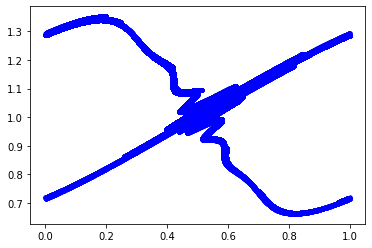
\includegraphics[width=0.5\textwidth,height=\textwidth,keepaspectratio]{images/7-c.png}
            \caption{Global unstable manifold in blue ran for 22 iterations.}
        \end{figure}
        
        To achieve this we used the following code: 
        \begin{python}
    num_iterations=22
    x1_unstable_array=np.zeros([x1_ic_unstable_list.shape[0],num_iterations])
    x2_unstable_array=np.zeros(x1_unstable_array.shape)

    for ic in np.arange(num_ics):
        x1_unstable_array[ic,0]=x1_ic_unstable_list[ic]
        x2_unstable_array[ic,0]=x2_ic_unstable_list[ic]        
        for n in np.arange(num_iterations-1):    
            x1_unstable_array[ic,n+1]=f_fun(x1_unstable_array[ic,n],x2_unstable_array[ic,n])
            x2_unstable_array[ic,n+1]=g_fun(x1_unstable_array[ic,n],x2_unstable_array[ic,n])

    plt.figure()
    for n in np.arange(num_iterations):    
        plt.plot(x1_unstable_array[:,n],x2_unstable_array[:,n],'.',color='blue',label="unstable manif.")
    plt.show()
        \end{python}




        \item [(d)]
        Next we wish to construct the inverse map. Observe that since
        \[ 
            I_{n+1} = I_n + - \frac{1}{2\pi} \sin(2\pi \theta_n) \implies I_n = I_{n+1} + \frac{1}{2\pi}\sin(2\pi \theta_n)
        \]
        and plugging this into the $\theta_{n+1}$ equation yields
        \[ 
            \theta_{n+1} = \theta_{n} + I_{n+1} \bmod 1.
        \]
        Thus we have found the inverse map to be
        \[ 
            \begin{cases}
                \theta_n = \theta_{n+1} - I_{n+1} \bmod 1,\\
                I_n = I_{n+1} + \frac{1}{2\pi}\sin(2\pi (\theta_{n+1} - I_{n+1})).
            \end{cases}
        \]




        \item [(e)]
        Now that we have found the inverse map, we wish to find a view of the global structure of the global stable manifold. To achieve this, we use the same set up as shown in part (c) but now use the inverse map and stable eigenspace. Using $N=22$ iterations, we see that the global stable manifold in the following plot:  
        \begin{figure}[H]
            \centering
            \hspace*{0cm}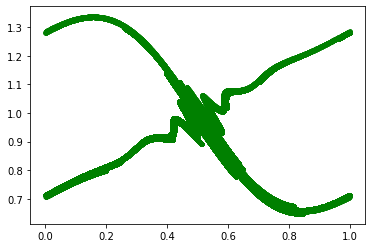
\includegraphics[width=0.5\textwidth,height=\textwidth,keepaspectratio]{images/7-e.png}
            \caption{Global stable manifold in green ran for 22 iterations.}
        \end{figure}
        
        To achieve this we used the following code: 
        \begin{python}
    num_iterations=22
    x1_stable_array=np.zeros([x1_ic_stable_list.shape[0],num_iterations])
    x2_stable_array=np.zeros(x1_stable_array.shape)
    
    for ic in np.arange(num_ics):
        x1_stable_array[ic,0]=x1_ic_stable_list[ic]
        x2_stable_array[ic,0]=x2_ic_stable_list[ic]
        
        for n in np.arange(num_iterations-1):    
            x1_stable_array[ic,n+1]=f_inv_fun(x1_stable_array[ic,n],x2_stable_array[ic,n])
            x2_stable_array[ic,n+1]=g_inv_fun(x1_stable_array[ic,n],x2_stable_array[ic,n])
    
    plt.figure()
    for n in np.arange(num_iterations):    
        plt.plot(x1_stable_array[:,n],x2_stable_array[:,n],'.',color='green',label="stable manif.")
    plt.show()
        \end{python}



        \item [(f)]
        Next we wish to view the homoclinic tangle of both the stable and unstable manifolds. We found that $N=30$ iterations was sufficient to see the structure of the homoclinic tangle. Using the provided in part (c) and part (e) we generate the following graph:
        \begin{figure}[H]
            \centering
            \hspace*{0cm}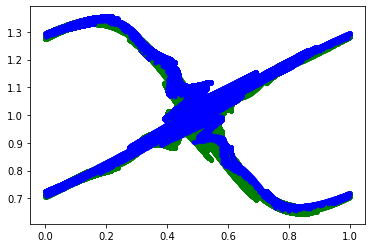
\includegraphics[width=0.5\textwidth,height=\textwidth,keepaspectratio]{images/7-f.png}
            \caption{Homoclinic tangle of both the stable (seen in green) and unstable (seen in blue) manifold ran for $30$ iterations.}
        \end{figure}
        
        
        \item [(g)]
        Finally we will pick a single point within the homoclinic tangle that is close to the fixed point and follow its trajectory throughout the iterations. To achieve this, we pick a random initial condition that is close to the fixed point, let's say the $14$th element of the unstable initial conditions $(0.5000000650032501, 1.000000040174218)$ and apply the map to the point. Doing so and plotting the trajectory of the point and the homoclinic tangle yields the following plot
        \begin{figure}[H]
            \centering
            \hspace*{0cm}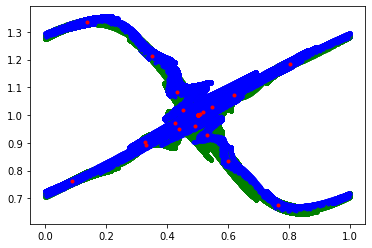
\includegraphics[width=0.5\textwidth,height=\textwidth,keepaspectratio]{images/7-g.png}
            \caption{Homoclinic tangle of both the stable (seen in green) and unstable (seen in blue) manifold ran and trajectory of the point $(0.5000000650032501, 1.000000040174218)$ (seen in red) for $30$ iterations.}
        \end{figure}
        We can see that the point begins near the origin and since the manifold is tangent to the eigenvectors defining the stable and unstable linear eigenspace, the point is shot out along one of the eigenvectors. The point travels back towards the fixed point and repeats the process. 


        To achieve this we used the following code: 
        \begin{python}
    num_iterations=30
    trajectoryIndex = 13;

    trajectoryX = np.zeros(num_iterations)
    trajectoryY = np.zeros(num_iterations)

    trajectoryX[0] = x1_ic_unstable_list[trajectoryIndex];
    trajectoryY[0] = x2_ic_unstable_list[trajectoryIndex];

    for n in range(num_iterations-1):
        trajectoryX[n+1] = f_fun(trajectoryX[n],trajectoryY[n])
        trajectoryY[n+1] = g_fun(trajectoryX[n],trajectoryY[n])
        \end{python} 
    
    
    \end{enumerate}


\end{solution}

%----------------------------------------------------------------------------------------------------%
%\vskip 20pt
\newpage

%---------------%
%---Problem 8---%
%---------------%

%--status--$

\begin{problem}
    Yeast cells break down
sugar by glycolysis, and there is a simple model for this:
\begin{equation}
\left\{\begin{array}{l}
\dot{x}=-x+a y+x^{2} y \equiv f(x, y) \\
\dot{y}=b-a y-x^{2} y \equiv g(x, y)
\end{array}\right.
\end{equation}
where x represents ADP adenosine diphosphate and y is F6P fructose-6-phosphate
concentrations $(x , y \ge 0)$. Assume $0 < a \le 1/8$. By constructing a trapping region
and using Poincare-Bendixson theorem, find the range of b where one can guarantee
the existence of a stable periodic orbit.  Hint:  you may wish to plot the vectorfield using the ipython notebook form class, or pplane (matlab) or other software, to get inspiration for where you would like to define the trapping region. 
\end{problem}

\begin{figure}
    \centering
    \hspace*{0cm}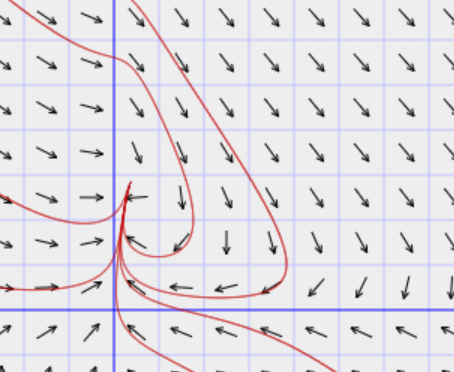
\includegraphics[width=0.4\textwidth,height=\textwidth,keepaspectratio]{images/8-sup.PNG}
    \caption{Phase portrait of system (9) with $a=0.1$ and $b=0.2$.}
\end{figure}


\begin{solution}
    \noindent
    Consider the system
    \begin{equation*}
        \left\{\begin{array}{l}
        \dot{x}=-x+a y+x^{2} y  \\
        \dot{y}=b-a y-x^{2} y 
        \end{array}\right.,
    \end{equation*}
    for $0 \leq a \leq \frac{1}{8}$ and $x,y \geq 0$. We wish to construct a trapping region and use Poincare-Bendixson theorem to find a range of $b$ such that we can guarantee the existence of a stable periodic orbit. We begin by finding the nullclines of the systems by setting $x' =0$ and $y'=0$. thus we have the nullclines to be defined by
    \[
        \begin{cases}
            \dot{x}=-x+a y+x^{2} y = 0\\
            \dot{y}=b-a y-x^{2} y = 0
        \end{cases} \implies \begin{cases}
            y = x/(a+x^2)\\
            y = b/(a+x^2).      
        \end{cases}
    \]
    Sketching the nullclines along with a vector field of the system generated in Mathematica, see Figure 5, we claim there exists a trapping region as defined in the following sketch:
    \begin{figure}[H]
        \centering
        \hspace*{0cm}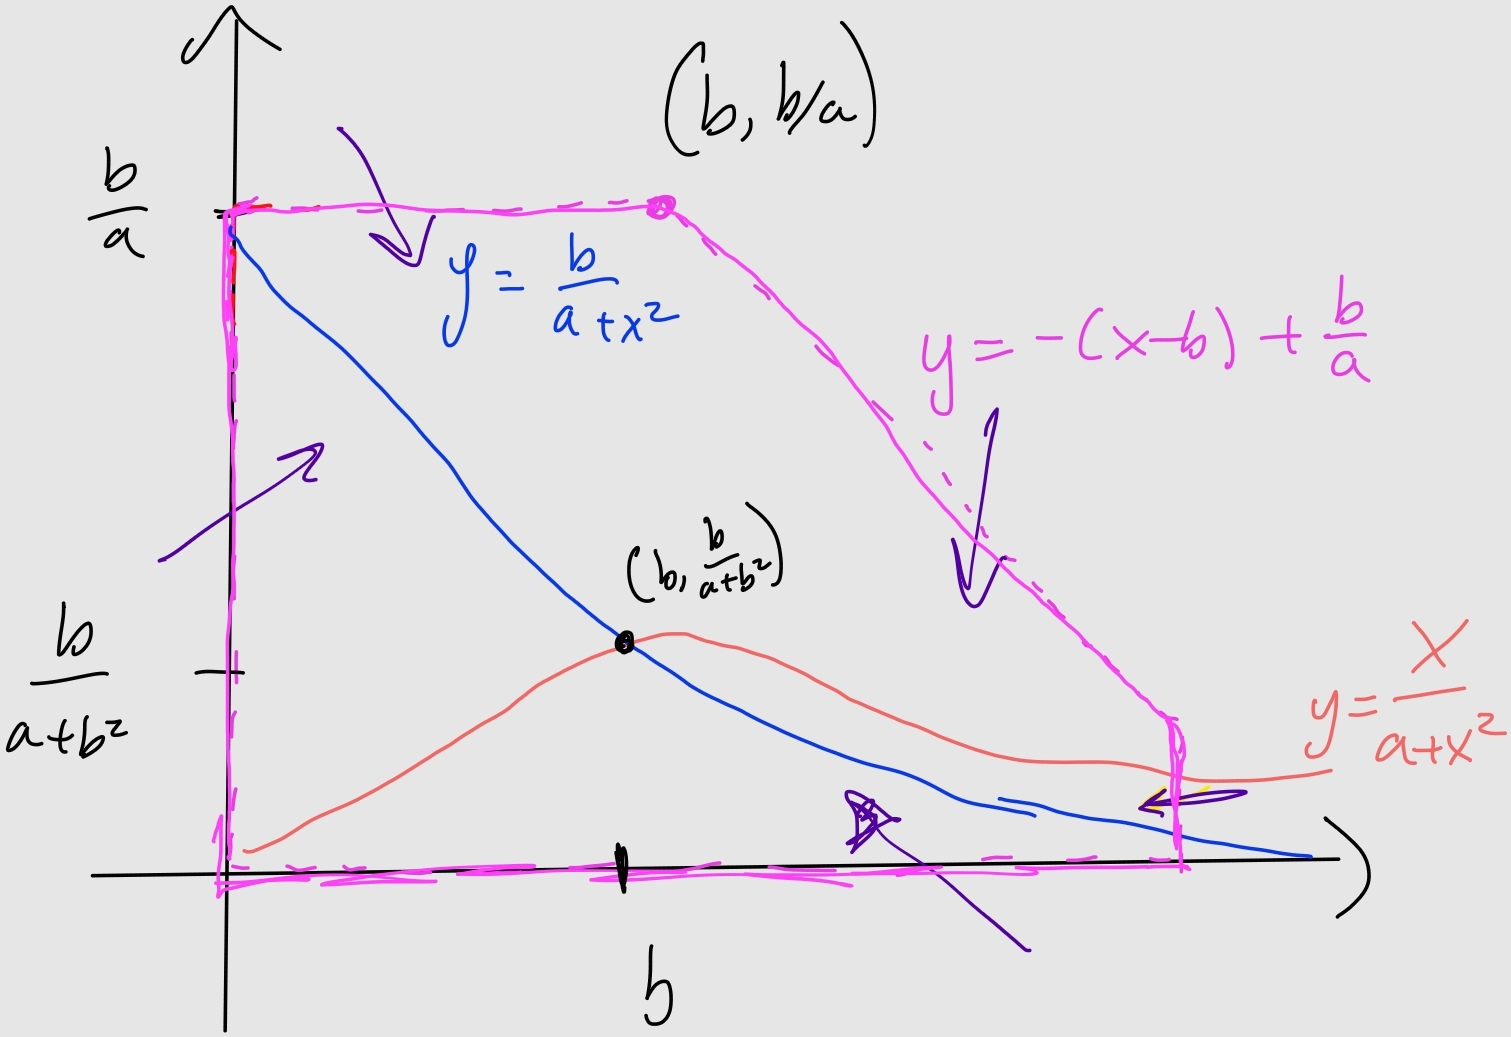
\includegraphics[width=0.5\textwidth,height=\textwidth,keepaspectratio]{images/8.jpg}
        \caption{Trapping region seen in pink. Purple arrows show flow of vector field determined by Figure 5.}
    \end{figure} 
    We can verify the direction along the line $y = -(x-b) + \frac{b}{a}$ by observing that
    \[
        \frac{y'}{x'} < -1 \implies y' + x' < 0 \implies b - x < 0 \implies x > b,
    \]
    which is true along the line by construction. Thus the region is indeed trapping. To satisfy Poincare-Bendixson theorem, we need to remove the fixed point (at the intersection of the nullclines $(b,\frac{b}{a+b^2})$) from the trapped region and ensure that the fixed point is unstable. We an cut a neighborhood out of the trapping region and to find the stability of the fixed point, we will compute the Jacobian to be
    \[
         J(x,y) = \begin{bmatrix}
            -1 + 2xy & a + x^2\\
            -2xy & -a - x^2
         \end{bmatrix},
    \]
    and evaluating the jacobian at the fixed point we see
    \[ 
        J\paren{b,\frac{b}{a+b^2}} = \begin{bmatrix}
            -1 + \frac{2b^2}{a + b^2} & a + b^2\\
            \frac{-2b^2}{a + b^2} & - a - b^2.
        \end{bmatrix}
    \]
    The determinant of this matrix is given by
    \[ 
        \text{Det}\left( J\paren{b,\frac{b}{a+b^2}} \right) = -\frac{2 a b^2}{a+b^2}-\frac{2 b^4}{a+b^2}+a+3 b^2 = a + b^2
    \]
    and the trace of the matrix is given by 
    \[ 
        \text{Tr}\left( J\paren{b,\frac{b}{a+b^2}} \right) = \frac{2 b^2}{a+b^2}-a-b^2-1 = \frac{-(a+b^2) - (a + b^2)^2 + 2b^2}{a + b^2}.
    \]
    We know that if both the determinant and trace are positive, than so are the eigenvalues. We clearly see that the determinant is positive so let's restrict the trace to be positive,  
    \[ 
        -(a+b^2) - (a + b^2)^2 + 2b^2 > 0.
    \]
    To find the range of $b$, let's set the inequality to an equality and solve for $b$ which gives,
    \[ 
        b = \pm \paren{ \frac{1}{2} \paren{1 - 2a \pm \sqrt{1 - 8 a}}}^{1/2},
    \]
    and setting $a = \frac{1}{8}$ we find that in order for the trace to be positive, $b \in \paren{-\sqrt{\frac{3}{8}},\sqrt{\frac{3}{8}}}$. Thus if we restrict $b$ to be in this range and remove the fixed point from the trapping region, by Poincare-Bendixson we are guarantee the existence of stable periodic orbit.



\end{solution}

%----------------------------------------------------------------------------------------------------%
%\vskip 20pt
\newpage

%---------------%
%---Problem 9---%
%---------------%

%--status--$

\begin{problem}
    Consider the system
\begin{equation}
\left\{\begin{array}{l}
\dot{x}=x(a-by) \\
\dot{y}=y(-c+dx)
\end{array}\right.
\end{equation}
where the parameters $a,b,c,d$ are all assumed to be positive. Additionally, since we are dealing with populations, we only consider $x,y \geq 0$.\\

\begin{enumerate}
    
\item[(a)] Find the fixed points of this system, and determine whether they are lyapunov stable, asymptotically stable, or inconclusive based on the eigenvalues (i.e. the linearized system).

\item[(b)] Draw the $x$-nullclines and the $y$-nullclines of the system. They should separate the region $x,y>0$ into four basic regions. Add a rough sketch of the vector fields in each of these regions to your drawing. What can you infer about the solutions of this system? 

\item[(c)] Next, let us search for a Lyapunov function $L$ for the system. Using the trick of {\it separation of variables}, we will look for a function of the form
\begin{equation}
    L(x,y) = F(x) + G(y).
\end{equation}
Additionally, we will use the facts that $dL/dt := 0$ along solutions of the system, and that $x$ and $y$ are independent variables to obtain solvable ODEs for $F(x)$ and $G(y)$. \\

\item[(d)] Finally, use the Lyapunov function to answer any remaining questions about the stability of the fixed points of our original system. (Note that strictly speaking the function $L(x,y)$ that you obtain might need to be shifted by a constant value to make it a true a Lyapunov function.) 

\end{enumerate}

\end{problem}

\begin{solution}

    \noindent
    Consider the system
    \begin{equation}
        \left\{\begin{array}{l}
        \dot{x}=x(a-by) \\
        \dot{y}=y(-c+dx)
        \end{array}\right.
    \end{equation}
    where the parameters $a,b,c,c$ are all assumed to be positive. Additionally, since we are dealing with populations, we only consider $x,y \geq 0$. 

    \begin{enumerate}
        \item [(a)]
            We first find the fixed points by setting $\dot x = \dot y = 0$ which gives the two fixed points
            \[ 
                (0,0) \and \left(\frac{c}{d},\frac{a}{b}\right).
            \]
            Next we will find the Jacobian to be
            \[ 
                J(x,y) = \left(
                    \begin{array}{cc}
                     a-b y & -b x \\
                     d y & d x-c \\
                    \end{array}
                    \right),
            \] 
            and evaluating the Jacobian at $(0,0)$ yields
            \[ 
                J(0,0) = \left(
                    \begin{array}{cc}
                     a & 0 \\
                     0 & -c \\
                    \end{array}
                    \right)
            \]
            which has eigenvalues $\lambda_1 = a$ and $\lambda_2 = -c$. Thus the origin is unstable since $\text{Re}\left(\lambda_1\right) > 0$. Next we evaluate the Jacobian at $ \left(\frac{c}{d},\frac{a}{b}\right)$ which gives
            \[ 
                J\left(\frac{c}{d},\frac{a}{b}\right) = \left(
                    \begin{array}{cc}
                     0 & -\frac{b c}{d} \\
                     \frac{a d}{b} & 0 \\
                    \end{array}
                    \right), 
            \] 
            which have eigenvalues $\lambda_{1,2} = \pm i \sqrt{ac}$. Thus the fixed point $\left(\frac{c}{d},\frac{a}{b}\right)$ is inconclusive since $\text{Re}(\lambda_1) = \text{Re}(\lambda_2) = 0$. 


        \item [(b)]
            Next we wish to the $x$-nullclines which is when $\dot x = 0$ and thus we have that
            \[ 
                \dot x = 0 \implies x(a - by)=0
            \]
            and thus we have that $x=0$ and $y=a/b$ which define the $x$-nullclines. Similarly we find that the $y$-nullclines which is when $\dot y = 0$. and thus we have that
            \[ 
                \dot y = 0 \implies y(-c+dx) = 0,
            \] 
            and thus we have that $y=0$ and $x=c/d$ define the $y$-nullclines. Drawing the nullclines (seen in red) on top of a phase portrait of our system with $a=7.21906, b=3.79283, c=4.65532, \and d=3.48126$ we see the following graph:
            \begin{figure}[H]
                \centering
                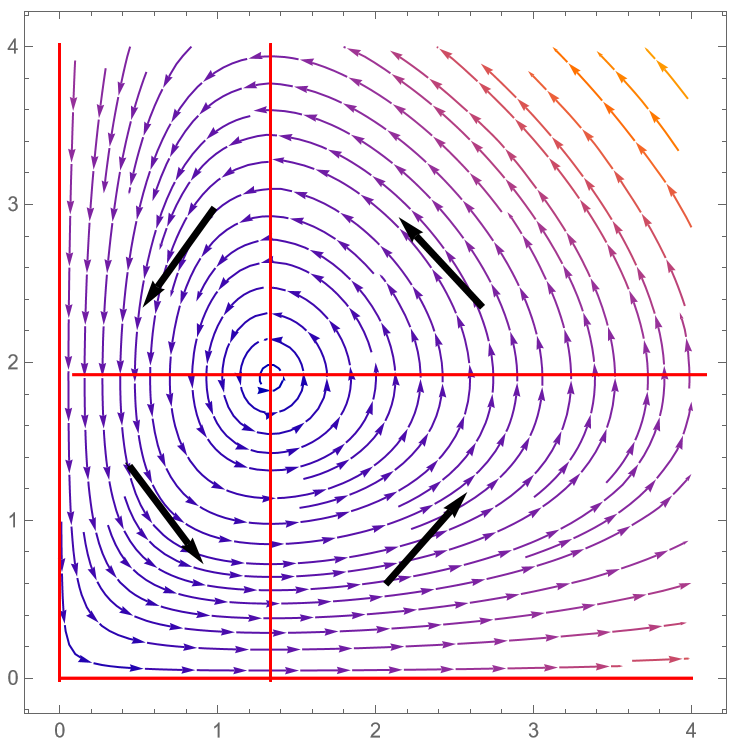
\includegraphics[width=0.5\textwidth,height=\textwidth,keepaspectratio]{images/9-b-1.png}
                \label{fig9}
            \end{figure}
            where we can see that the solution is oscillatory about the fixed point at $\left(\frac{c}{d},\frac{a}{b}\right)$ as all trajectories in each region follow the direction indicated by the black arrow. 



        \item [(c)]
            Now we wish to find a Lyapunov function $L$. Using separation of variable, we will look for a function of the form
            \[ 
                L(x,y) = F(x) + G(y),
            \]
            noting that $\dd{L}{t} = 0$. Observe that we have
            \[ 
                0 = \dd{L}{t} = F'(x)(x(a-by)) + G'(y)(y(-c + dx)),
            \]
            and moving all the terms with $y$ to one side and the terms with $x$ to other we get
            \[ 
                F'(x) \paren{\frac{x}{c - dx}} = G'\paren{\frac{y}{a-by}} = \Lambda,
            \]
            where $\Lambda$ is some real constant. Let's first consider when
            \[ 
                F'(x)  = \Lambda\paren{\frac{c - dx}{x}},
            \]
            and integrating both sides we find that
            \[ 
                F(x) = \Lambda\paren{c \ln(x) - dx + C_1}.
            \]
            Similarly, we find that
            \[ 
                G(y) = \Lambda\paren{a \ln(y) - by + C_2},
            \] 
            which gives
            \[ 
                L = \Lambda\paren{c \ln(x) - dx + \ln(y) - by + C_3}.
            \]
            Now we can enforce that $L\left(\frac{c}{d},\frac{a}{b}\right) = 0$ which gives
            \[ 
            L\left(\frac{c}{d},\frac{a}{b}\right) = \Lambda\paren{c \ln\left(\frac{c}{d}\right) - c + a\ln\left(\frac{a}{b}\right) - a + C_3} = 0,
            \]
            and thus we have found that
            \[ 
                C_3 = -c \ln\left(\frac{c}{d}\right) + c - \ln\left(\frac{a}{b}\right) + a. 
            \]
            Therefore 
            \[
                L = \Lambda\paren{c \ln\paren{\frac{dx}{c}} + (c - dx) + a\ln\paren{\frac{by}{a}} + (a- by)}.
            \]
            For $L$ to be Lyapunov, the remaining condition to be shown is that $L(x,y) > 0$ for $(x,y) \neq \left(\frac{c}{d},\frac{a}{b}\right)$. Observe that if we set $x= \frac{c}{d} + \tilde{x}$ and $y = \frac{a}{b} + \tilde{y}$ we have,
            \[ 
                L(\tilde{x},\tilde{y}) = \Lambda\paren{c \ln\paren{1 + \frac{d\tilde{x}}{c}} - d\tilde{x} + a\ln\paren{1 + \frac{b\tilde{y}}{a}} - b\tilde{y}}.
            \]
            Let's first consider when $\Lambda < 0$, we require that 
            \[ 
                \Lambda\paren{c \ln\paren{1 + \frac{d\tilde{x}}{c}} - d\tilde{x}} + \Lambda \paren{a\ln\paren{1 + \frac{b\tilde{y}}{a}} - b\tilde{y}} > 0,
            \]
            let's study the first term first. Observe that
            \begin{align*}
                \Lambda\paren{c \ln\paren{1 + \frac{d\tilde{x}}{c}} - d\tilde{x}} &> 0\\
                c \ln\paren{1 + \frac{d\tilde{x}}{c}} - d\tilde{x} &< 0\\
                1 + \frac{d\tilde{x}}{c} &< \exp\paren{\frac{d\tilde{x}}{c}},
            \end{align*} 
            and Taylor expanding we get that
            \begin{align*}
                1 + \frac{d\tilde{x}}{c} &< 1 + \frac{d\tilde{x}}{c} + \paren{\frac{d\tilde{x}}{c}}^2 + O(\tilde{x}^3)\\
                0 &< \paren{\frac{d\tilde{x}}{c}}^2 + O(\tilde{x}^3),
            \end{align*}
            which is satisfied for sufficiently small $\tilde{x}$. We can make a similar argument for the second term and a sufficiently small $\tilde{y}$ term. In the case when $\Lambda > 0$, the inequality will be flipped and clearly not be satisfied. Thus in a local neighborhood around the fixed point with $\Lambda < 0$, $L$ is a Lyapunov function. 
        \item [(d)]
            In part (c) we found a Lyapunov function for the fixed point and thus the fixed point is lyapunov stable. 
    
    
    \end{enumerate}



\end{solution}

%----------------------------------------------------------------------------------------------------%
%\vskip 20pt
\newpage


\end{document}